\documentclass{article}

% \usepackage{showframe}
% \usepackage[export]{adjustbox}
% \usepackage[a4paper, vmargin=1in]{geometry}
\usepackage{graphicx}
\usepackage{polski}
\usepackage{indentfirst}
\usepackage{fancyhdr}
\usepackage{float}
\usepackage{subcaption}
\usepackage{multirow}
\usepackage{hyperref}

\pagestyle{fancy}
\fancyhf{}

\lhead{Architektura Komputerów 2}
\rhead{\thepage}

\begin{document}

% strona tytułowa
\begin{titlepage}
	\clearpage
	\thispagestyle{empty}
	\pagenumbering{gobble}
    \centering
    
	{\LARGE Architektura Komputerów 2 \par}
	
	\vspace{1.5cm}
	
	{\huge\bfseries Liczby zdenormalizowane\par}
	
	\vspace{1.5cm}
	{\large czwartek nieparzysty, 18:55\par}

	\vspace{1cm}
    \parbox{0.4\linewidth}{
	    \centering
	    {\Large Michał \textsc{Sieroń}\par}
	    {\large 256 259\par}
	}
    \hfill
    \parbox{0.4\linewidth}{
	    \centering
	    {\Large Paweł \textsc{Różański}\par}
	    {\large 252 772\par}
	}

	\vspace{1.5cm}
	{\large prowadzący\par}
	{\large dr inż. Piotr \textsc{Patronik}\par}
    
	\vfill

	{\large Informatyka Techniczna, Wydział Elektroniki\par}
	\vspace{0.5cm}
	{\large \today\par}
	\clearpage
	\pagenumbering{arabic}
\end{titlepage}

\tableofcontents
\newpage

\section{Wstęp}
Zadanie projektowe polegało na analizie zawartości artykułu i implementacji przedstawionych układów w języku \emph{Verilog}.
Z powodu ograniczonego czasu na wykonanie projektu możliwe było zaimplemenetowanie jedynie układów \emph{A1} oraz \emph{M} przedstawionych w artykule \cite{art:old}.

Następnie zaimplementowano odpowiadajace im układy zgodne ze standardem \emph{IEEE-754} \cite{art:ieee754}.
Dokonano również porównania błędów wynikajacych z użycia danej reprezentacji liczby zmiennoprzecinkowej. 


\section{Opis koncepcji zapisu i formatu}
Koncepcja formatu liczb zmiennoporzecinkowych, zaproponowanego w artykule \cite{art:old} wzięła się z~obserwacji, że standard \emph{IEEE-754} nie został stworzony z myślą o systemach wbudowanych.
Eliminacja logiki normalizującej powinna obniżyć koszt produkcji układu, a wpływ na precyzję obliczeń nie powinien mieć znaczenia w docelowych zastosowaniach.
Normalizacja liczby jest sktukiem używania ukrytej jedynki w liczbach znormalizowanych.
Sprawia to, że pojawia się wyjątek, który trzeba obsłużyć w sprzęcie.
Proponowany format pozbywa się ukrytej jedynki, kosztem jednego z bitów mantysy.
Konsekwencją tego jest zmniejszona precyzja liczb.


\section{Opis metody}
Wszystkie układy zostały zaimplementowane w języku opisu sprzętu \emph{Verilog}.
Jednak druga część projektu, która je ze sobą łączy i porównuje z wartością referencyjną, została napisana w języku \emph{Python}.
Dla zadanej ilości przypadków testowych generowaliśmy tyle samo par liczb typu \texttt{float}.
W języku \emph{Python}, typ \texttt{float} odpowiada liczbie zmiennoprzecinkowej o podwójnej precyzji.
Wobec tego konieczne było przekonwertowanie wygenerowanych liczb na liczbę zmiennoprzecinkową o pojedynczej precyzji.
W tym celu napisaliśmy funkcję \texttt{py2float} w języku \emph{C}, która zamienia wartość typu \texttt{double} na \texttt{float}.
Tak otrzymane wartości były następnie zamieniane na ich szesnastkową reprezentację.
W tym celu musieliśmy uprzednio otrzymać bajtową reprezentację danej liczby, która z~kolei była zamieniana na liczbę typu \texttt{int}, z której w końcu mogliśmy otrzymać reprezentację w systemie szesnastkowym.

Konwersję z liczby znormalizowanej na zdenormalizowaną zaimplementowaliśmy w tym samym skrypcie.
W ten sam sposób co wcześniej, otrzymywaliśmy zapis szesnastkowy liczby lecz denormalizacja liczby wymaga operacji bitowych.
Przez fakt użycia \emph{Pythona} konieczne było do tego zamienienie liczby na listę bitów (w tym przypadku liczb całkowitych typu \texttt{int} o wartościach 0 lub 1).
Tak otrzymana lista była następnie odpowiednio dzielona na części znaku, wykładnika i mantysy.
Mantysa była przesuwana o jedną pozycję w prawo, a wykładnik zwiększany o jeden.
Tak zmodyfikowaną reprezentację bitową zamienialiśmy z~powrotem na zapis szesnastkowy.

Wykorzystując wygenerowane pary liczb tworzyliśmy pliki \emph{Veriloga} wykorzystujące napisane przez nas moduły opisane w sekcji \ref{sec:implementacja}.
Utworzone pliki były następnie uruchamiane, a wyniki zapisywane w pliku \emph{csv} do dalszego przetwarzania.


\section{Opis implementacji}\label{sec:implementacja}
Implementacja układu dodawania liczb zmiennoprzecinkowych została wykonana na podstawie opisu oraz 
modelu układu z artykułu \cite{art:old}.
Według nazewnictwa z artykułu układ dodawania, który odwzorowaliśmy, to \emph{A1}. 
Jest to najprostsza wersja dodawania dwóch liczb zdenormalizowanych.
% schemat dodawania zdenormalizowanego
\begin{figure}[H]
	\centering
	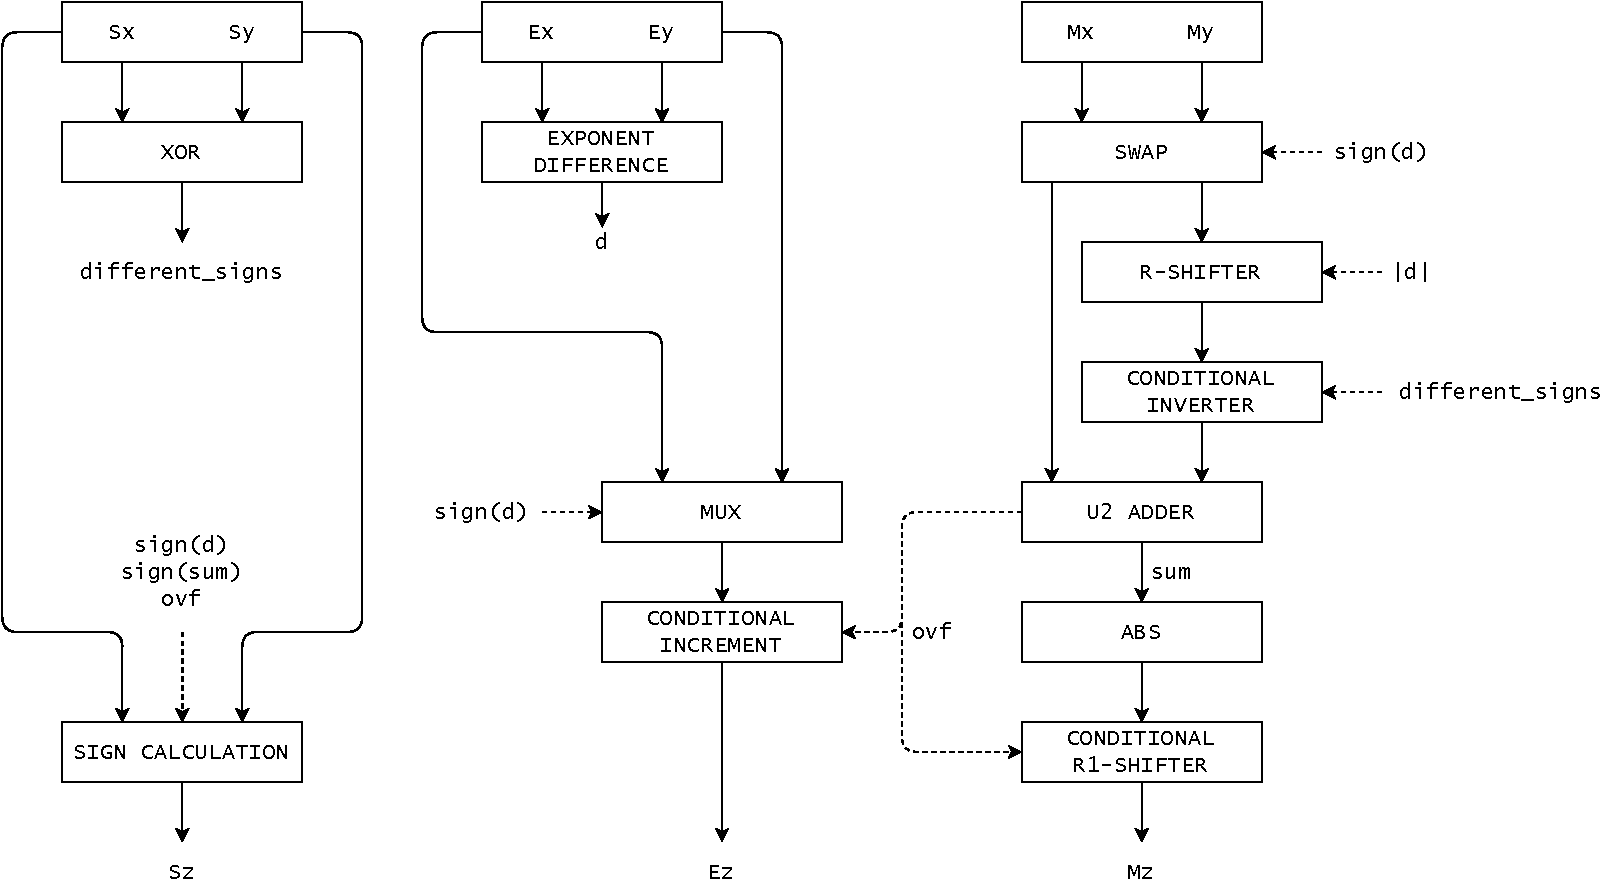
\includegraphics[width=\textwidth]{figures/diagram_add_denorm.pdf}
	\caption{Schemat układu dodawania - zdenormalizowane}
	\label{fig:diagram_add_denorm}
\end{figure}

% schemat dodawania IEEE-754
\begin{figure}[H]
	\centering
	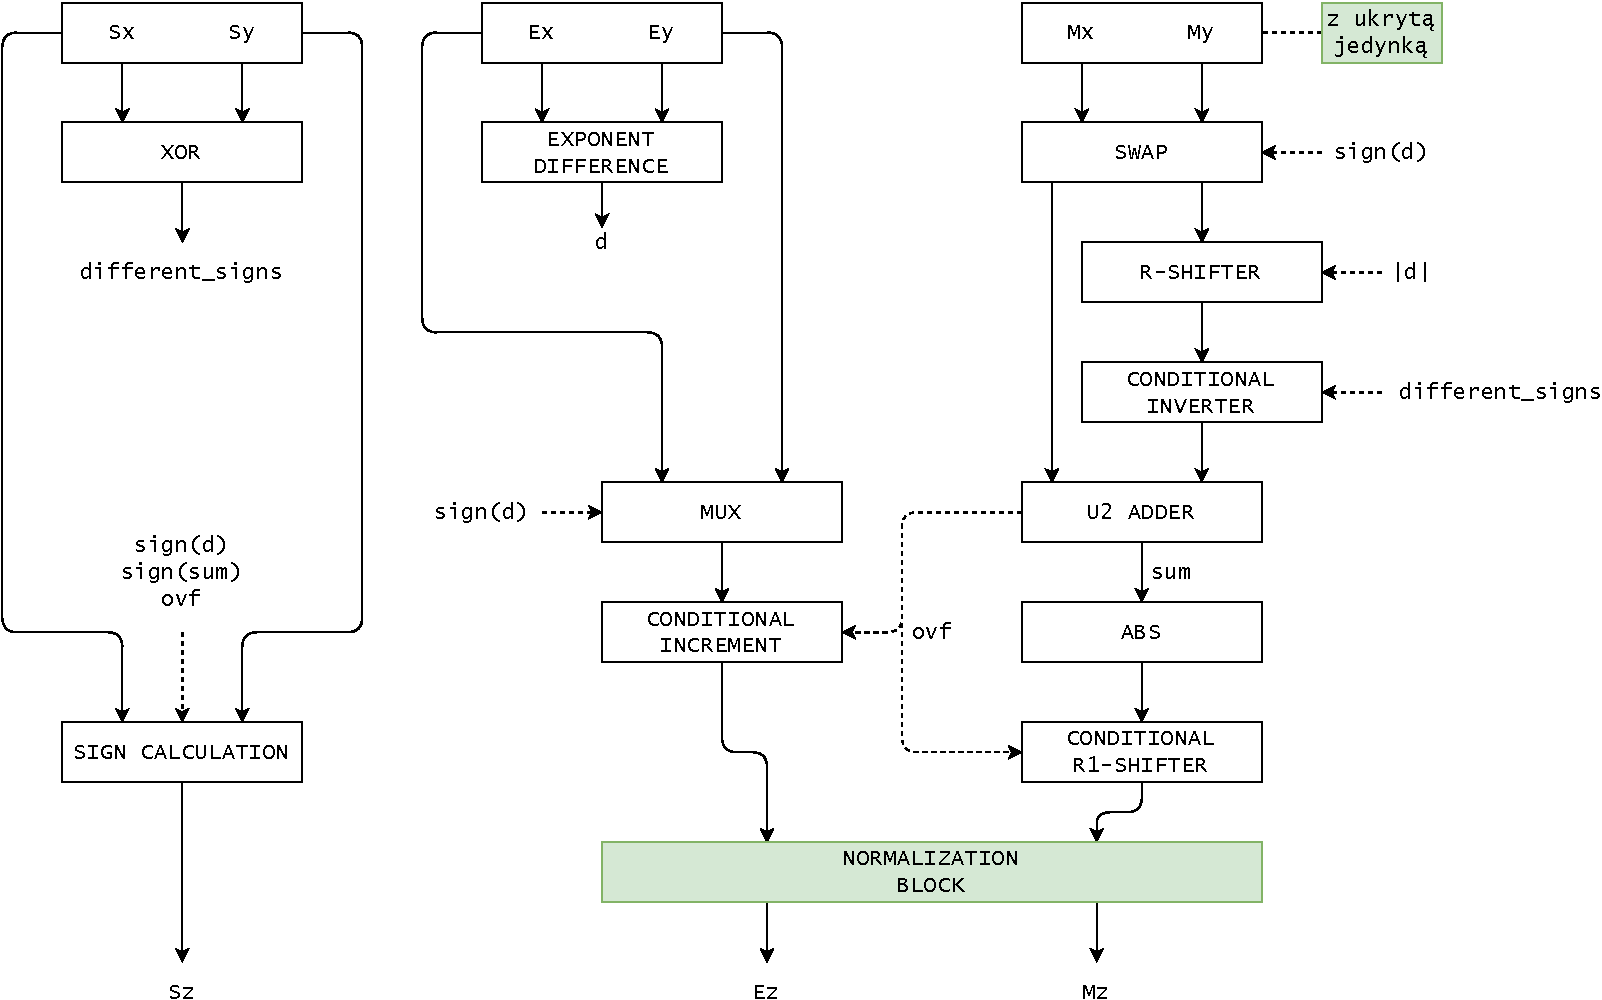
\includegraphics[width=\textwidth]{figures/diagram_add_ieee754.pdf}
	\caption{Schemat układu dodawania - \emph{IEEE-754}}
	\label{fig:diagram_add_ieee754}
\end{figure}
Autorzy nadali mu nazwę \emph{M}.
Jest to pierwsza zaproponowana przez autorów wersja implementacji układu mnożenia liczb zdenormalizowanych.
Podobnie jak układ dodawania, największą jego różnicą jest brak układu normalizacji wyniku.
Implemetancja układu mnożenia zdenormalizowanych liczb zmiennoprzecinkowych została wykonana w oparciu o diagram i opis układu \emph{M} w artykule.
W~architekturze, która została użyta w~układzie mnożenia, autorzy zakładają, że wynik mnożenia dwóch liczb zawsze zakończy się przepełnieniem, wobec tego wykładnik jest zawsze zwiększany jeden, a mantysa przesuwana  o jedna pozycję w prawo.

% schemat mnożenia zdenormalizowanego
\begin{figure}[H]
	\centering
	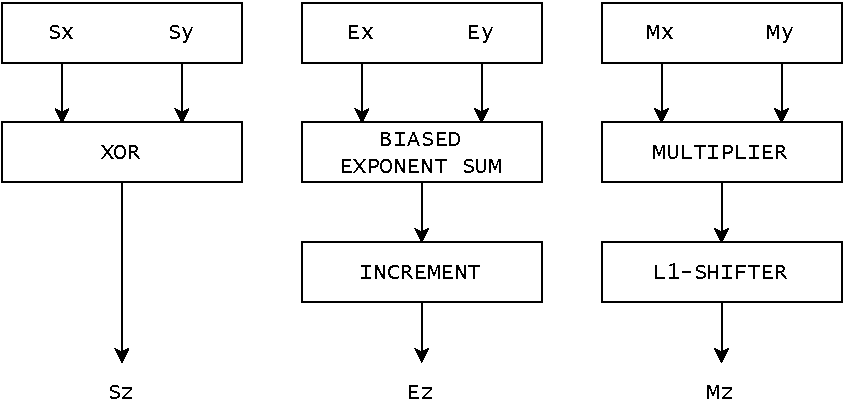
\includegraphics[width=\textwidth]{figures/diagram_mul_denorm.pdf}
	\caption{Schemat układu mnożenia - zdenormalizowane}
	\label{fig:diagram_mul_denorm}
\end{figure}

% schemat mnozenia IEEE-754
\begin{figure}[H]
	\centering
	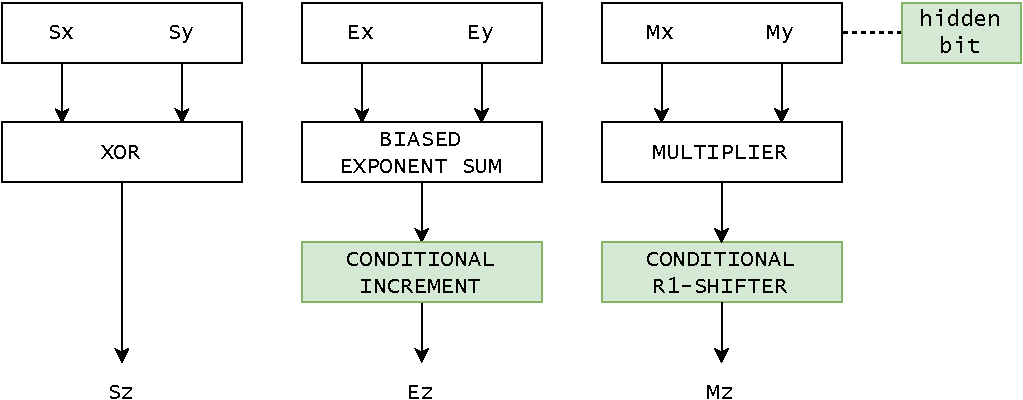
\includegraphics[width=\textwidth]{figures/diagram_mul_ieee754.pdf}
	\caption{Schemat układu mnożenia - \emph{IEEE-754}}
	\label{fig:diagram_mul_ieee754}
\end{figure}

\section{Różnice między metodami}

Wynika to z faktu, że gdy porównujemy tylko wykładniki może się zdażyć ze operand z wyższego wykładnika będzie mniejszy niż drugi. 
% Opis i schematy IEEE 754 porównanie

\section{Narzędzia}
Narzędziami, które zostały użyte przez znas są między innymi 3 języki programowania. Najbardziej korzystaliśmy z języka Verilog, który posłużył nam do łatwiejszej implementacji układów mnożenia i dodawania.
Języka C użyliśmy do implementacji układu porówania wyników a Pythona do przeprowadzenia wszystkich potrzebny testów wraz w wykonaniem wykresów obrazujących wyniki.
Przy implementacji z języku Verilog używaliśmy kompilatora iVerilog.
A do sprawdzenia poprawności wyników poszczególnych bloków i debugowania programu GTKWave.
Do utworzenia układów diagramów została użyta aplikacja Draw.io.
Całość kodu była tworzona w programie Visual Studio Code.
Kod był testowany wykonywany w subsystemie do systemu Windowsa (WSL).


% Użyte narzędzia

\section{Opis sposobu}
% (w jaki sposób zrobilismy to badanie) - w jaki sposób były liczone błędy, ilość kropeczek, czego użyliśmy do uzyskania wyników

\section{Wyniki pomiarów}
\begin{figure}[H]
	\centering
	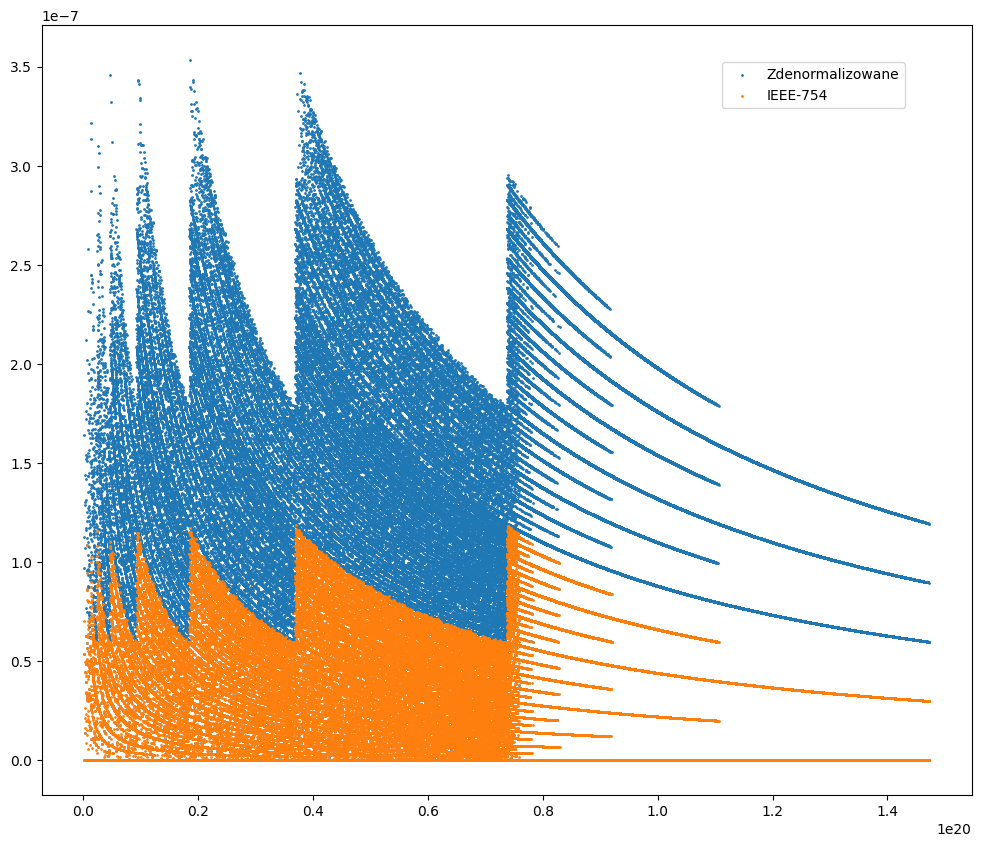
\includegraphics[height=0.4\textheight]{figures/add_relative.png}
	\caption{Błąd względny - dodawanie}
	\label{fig:add_relative}
\end{figure}

\begin{figure}[H]
	\centering
	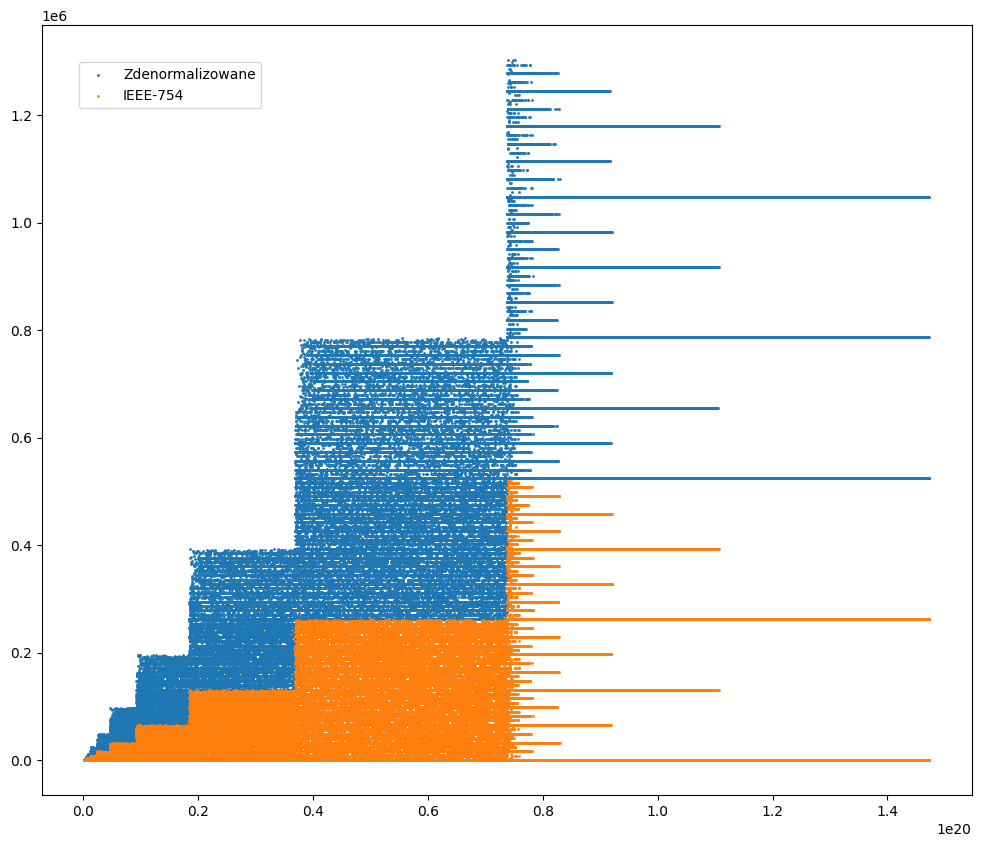
\includegraphics[height=0.4\textheight]{figures/add_ulp.png}
	\caption{Błąd bezwzględny - dodawanie}
	\label{fig:add_ulp}
\end{figure}


\begin{figure}[H]
	\centering
	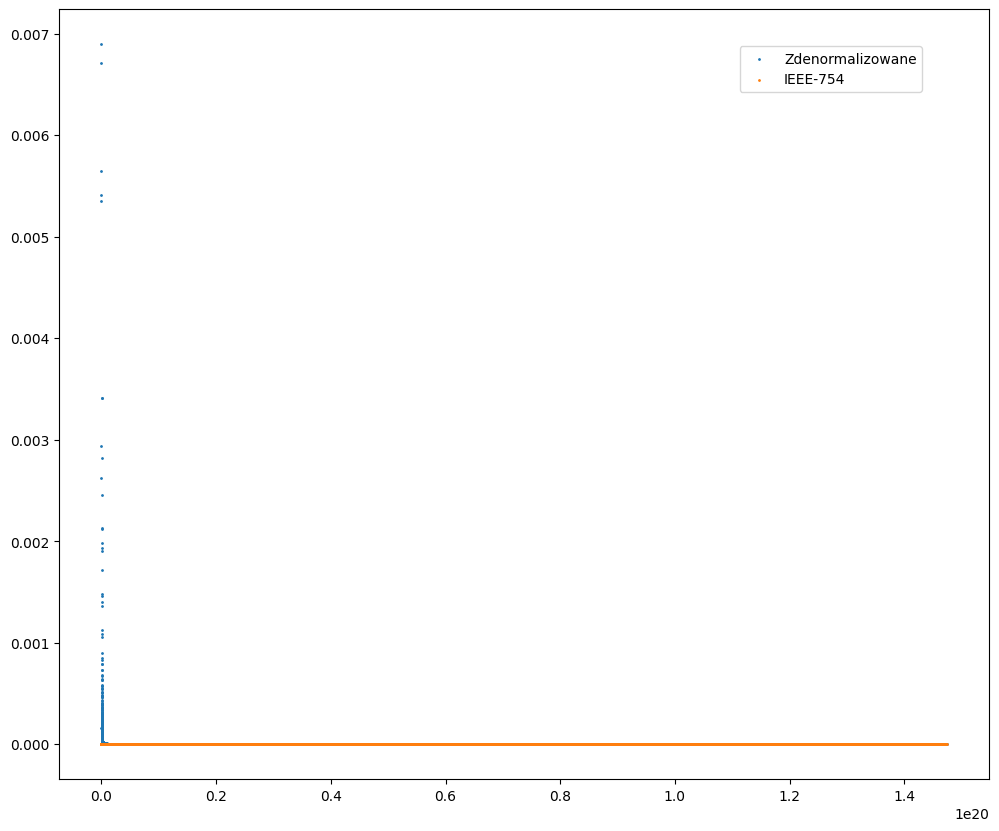
\includegraphics[height=0.4\textheight]{figures/sub_relative.png}
	\caption{Błąd względny - odejmowanie}
	\label{fig:sub_relative}
\end{figure}

\begin{figure}[H]
	\centering
	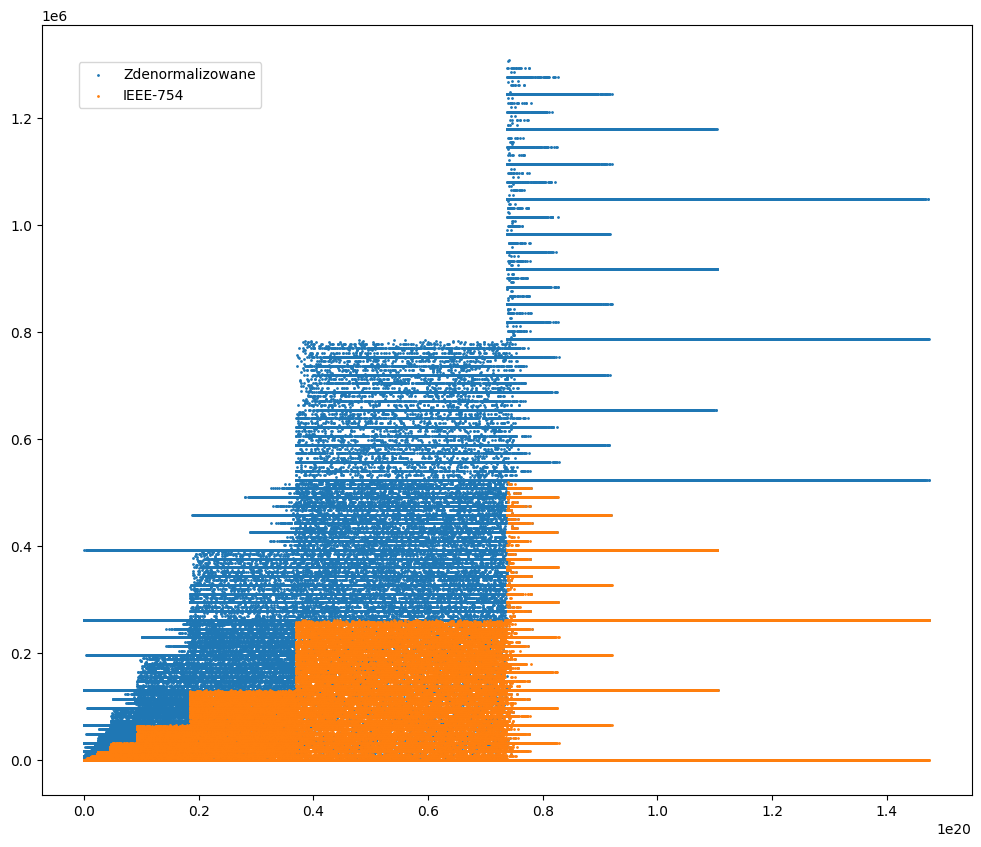
\includegraphics[height=0.4\textheight]{figures/sub_ulp.png}
	\caption{Błąd bezwzględny - odejmowanie}
	\label{fig:sub_ulp}
\end{figure}


\begin{figure}[H]
	\centering
	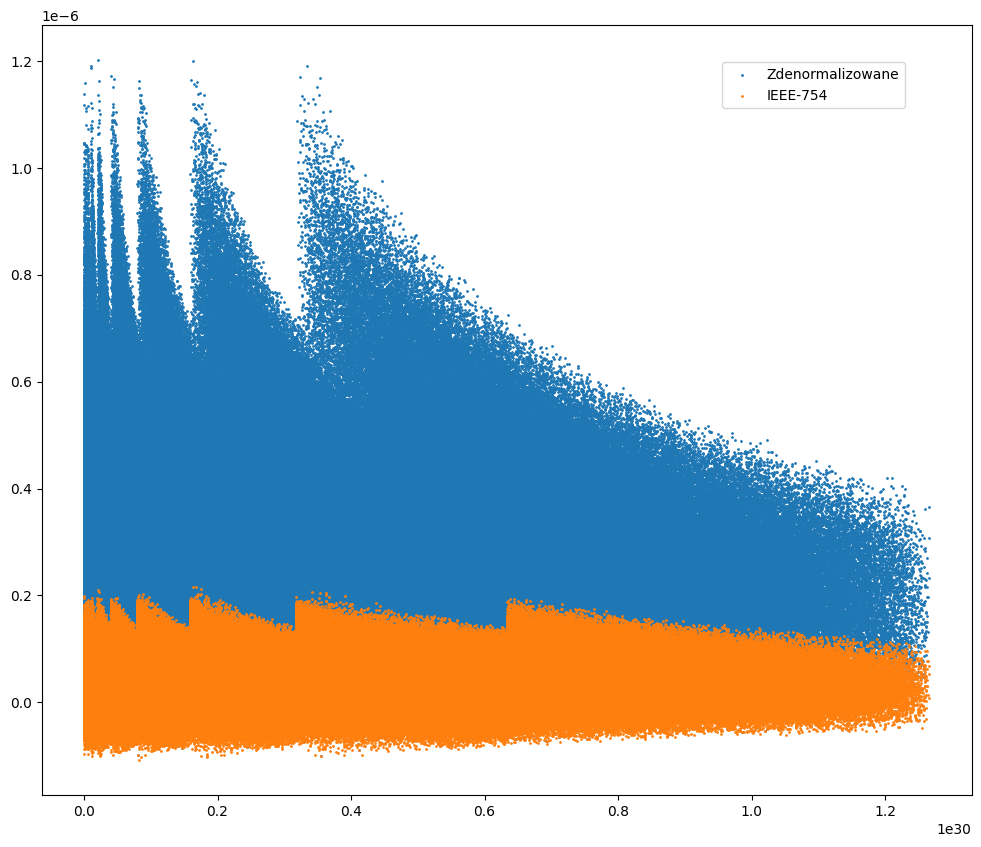
\includegraphics[height=0.4\textheight]{figures/mul_relative.png}
	\caption{Błąd względny - mnożenie}
	\label{fig:mul_relative}
\end{figure}

\begin{figure}[H]
	\centering
	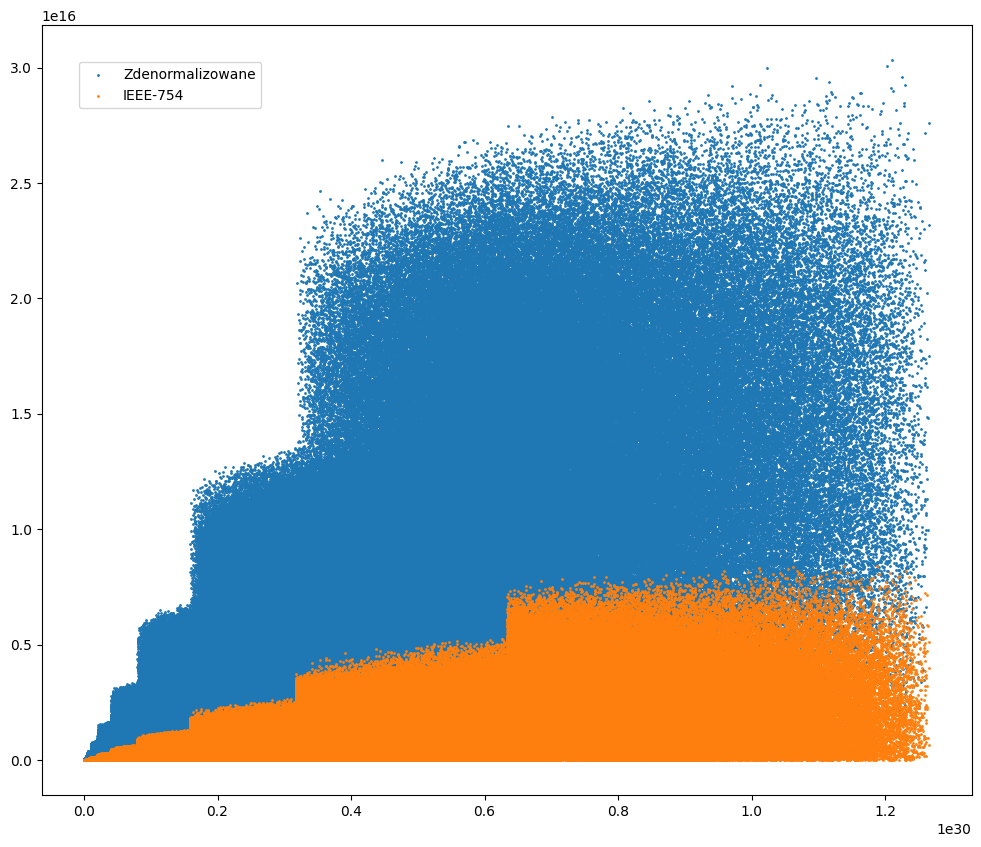
\includegraphics[height=0.4\textheight]{figures/mul_ulp.png}
	\caption{Błąd bezwzględny - mnożenie}
	\label{fig:mul_ulp}
\end{figure}

\section{Wnioski}


\newpage
\phantomsection
\addcontentsline{toc}{section}{Literatura}
\bibliography{bibliography}
\bibliographystyle{plabbrv}


\end{document}
